\documentclass[stu,11pt,spanish,floatsintext]{apa7}

%---------------------------------------------------------------------
% Idioma y codificación
%---------------------------------------------------------------------
\usepackage[spanish,es-tabla,es-noindentfirst]{babel}
\usepackage[utf8]{inputenc}
\usepackage[T1]{fontenc}
\usepackage{csquotes}

%---------------------------------------------------------------------
% Bibliografía en estilo APA (biblatex-apa)
%---------------------------------------------------------------------
\usepackage[style=apa,backend=biber]{biblatex}
\DeclareLanguageMapping{spanish}{spanish-apa}
\addbibresource{referencias.bib}

%---------------------------------------------------------------------
% Paquetes
%---------------------------------------------------------------------
\usepackage{graphicx}
\usepackage{float}
\usepackage{booktabs}
\usepackage{longtable}
\usepackage{array}
\usepackage{tabularx}
\usepackage{listings}
\usepackage{xcolor}
\usepackage{hyperref}
\usepackage{caption}

\graphicspath{{imagenes/}}

\hypersetup{
  colorlinks=true,
  linkcolor=black,
  citecolor=black,
  urlcolor=blue!60!black
}

\definecolor{codebg}{RGB}{245,245,245}
\definecolor{codekw}{RGB}{0,0,180}
\definecolor{codecomment}{RGB}{100,100,100}

\lstdefinestyle{terminal}{
  backgroundcolor=\color{codebg},
  basicstyle=\ttfamily\footnotesize,
  keywordstyle=\color{codekw}\bfseries,
  commentstyle=\color{codecomment}\itshape,
  breaklines=true,
  frame=single,
  rulecolor=\color{gray!40},
  numbers=left,
  numberstyle=\tiny\color{gray},
  captionpos=b,
  showstringspaces=false,
  tabsize=2,
  extendedchars=true,
  inputencoding=utf8,
  literate=%
    {á}{{\'a}}1 {é}{{\'e}}1 {í}{{\'i}}1 {ó}{{\'o}}1 {ú}{{\'u}}1
    {Á}{{\'A}}1 {É}{{\'E}}1 {Í}{{\'I}}1 {Ó}{{\'O}}1 {Ú}{{\'U}}1
    {ñ}{{\~n}}1 {Ñ}{{\~N}}1 {ü}{{\"u}}1 {Ü}{{\"U}}1 {¿}{{?`}}1 {¡}{{!`}}1
}
\lstset{style=terminal}

%=====================================================================
% METADATOS
%=====================================================================
\title{
  
\includegraphics[width=0.6\linewidth]{logo.png}\\[1cm]
  Evaluación conjunta: Auditoría de Seguridad y Despliegue en Kubernetes del Sistema InvenTrack
  }

\shorttitle{AUDITORÍA DE SEGURIDAD — INVENTRACK}

\author{Marcos Escobar}
\affiliation{Universidad de las Fuerzas Armadas ESPE}

\course{30735 — Desarrollo de Software Seguro}
\professor{Ing. Geovanny Cudco}
\duedate{31 de julio de 2026}

% \authornote{}

\begin{document}

\maketitle  

%=====================================================================
% RESUMEN (Abstract) — opcional en informes de estudiante.
%=====================================================================
% \begin{abstract}
% Resumen breve (150–250 palabras) del trabajo realizado: containerización,
% despliegue en Kubernetes bajo el dominio conjunta3p.espe.edu.ec y auditoría
% de seguridad PTES.
% \keywords{InvenTrack, Kubernetes, Docker, PTES, pentesting, APA 7}
% \end{abstract}

%=====================================================================
% ÍNDICE / TABLA DE CONTENIDO
%=====================================================================
\tableofcontents
\newpage

%=====================================================================
% 0. INTRODUCCIÓN
%=====================================================================
\section{Introducción}
El presente informe detalla el proceso de containerización, despliegue en un clúster de Kubernetes y auditoría de seguridad del sistema InvenTrack. Se documentan los pasos realizados para la creación de contenedores Docker para los componentes del sistema (backend, frontend y base de datos), la configuración de manifiestos de Kubernetes, el despliegue en un clúster local, y la configuración del Ingress para exponer la aplicación bajo el dominio \texttt{conjunta3p.espe.edu.ec}. Además, se presenta un análisis de seguridad siguiendo la metodología PTES (Penetration Testing Execution Standard), incluyendo la recopilación de inteligencia, modelado de amenazas, análisis de vulnerabilidades, explotación y post-explotación, así como las conclusiones y recomendaciones derivadas del proceso.

\subsection{Objetivo General}

El objetivo general de esta evaluación es realizar un despliegue seguro del sistema InvenTrack en un clúster de Kubernetes, asegurando la correcta containerización de sus componentes y evaluando su seguridad mediante pruebas de penetración siguiendo la metodología PTES. 

\subsection{Objetivos Específicos}
\begin{itemize}
  \item Realizar la containerización de los componentes del sistema InvenTrack (backend, frontend y base de datos) utilizando Docker.
  \item Configurar los manifiestos de Kubernetes necesarios para ejecutar InvenTrack en un clúster, incluyendo Deployments, Services, ConfigMaps, Secrets, PersistentVolumeClaims e Ingress.
  \item Configurar el Ingress para exponer la aplicación bajo el dominio \texttt{conjunta3p.espe.edu.ec} y asegurar la correcta resolución de DNS.
  \item Realizar una auditoría de seguridad del sistema InvenTrack siguiendo la metodología PTES, identificando vulnerabilidades y evaluando la efectividad de los controles de seguridad implementados.
\end{itemize}

\subsection{Enlace al Repositorio de Manifiestos de Kubernetes}
Repositorio GitHub (manifiestos \texttt{.yml}): \url{https://github.com/IMarcusDev/Evaluacion_Final_k8s_30735_DSS/tree/main}

%=====================================================================
% 1. DOCKERIZACIÓN DE COMPONENTES (10%)
%=====================================================================
\section{Dockerización de Componentes}

La containerización del sistema InvenTrack se organizó en tres componentes independientes: el backend (API REST en Node.js/Express), el frontend (aplicación React construida con Vite) y la base de datos MySQL. Para cada componente se definió una estrategia de empaquetado acorde con su función. El backend y el frontend se construyeron a partir de un \texttt{Dockerfile} propio, mientras que la base de datos se apoyó en la imagen oficial de MySQL 8.0, configurada por variables de entorno y volúmenes. En todos los casos se partió de imágenes base Alpine, que reducen el tamaño de la imagen resultante. A continuación se describen los Dockerfiles de cada componente y las decisiones de construcción aplicadas.

\subsection{Backend (Node.js/Express)}

\begin{lstlisting}[language=bash,caption={Dockerfile del Backend},label=lst:dockerbackend]
#Marcos Escobar
FROM node:20-alpine

WORKDIR /app

COPY package*.json ./
RUN npm ci --omit=dev

COPY . .

RUN mkdir -p uploads \
  && addgroup -g 1001 -S app \
  && adduser  -u 1001 -S app -G app \
  && chown -R app:app /app
USER app

EXPOSE 4000

CMD ["node", "src/app.js"]
\end{lstlisting}

El Dockerfile del backend, presentado en el Listado \ref{lst:dockerbackend}, partió de la imagen \texttt{node:20-alpine}. Primero se copiaron los archivos \texttt{package*.json} y se ejecutó \texttt{npm ci --omit=dev}, de modo que la imagen incorpora solo las dependencias de producción (--omit=dev es la versión moderna de --production). Después se copió el código fuente y se creó el directorio \texttt{uploads}, destinado a las imágenes de producto que gestiona Multer. Un aspecto relevante para la seguridad fue la creación de un usuario sin privilegios (\texttt{app}, con UID y GID 1001) y la asignación de la propiedad del directorio de trabajo a dicho usuario. La instrucción \texttt{USER app} evitó que el proceso se ejecute como \texttt{root} dentro del contenedor, lo que reduce el impacto de una eventual intrusión. Por último se expuso el puerto 4000 y se definió el arranque del servidor con \texttt{node src/app.js}.

\subsection{Frontend (React/Vite)}

\begin{lstlisting}[language=bash,caption={Dockerfile del Frontend (multi-stage)},label=lst:dockerfrontend]
#Marcos Escobar
FROM node:20-alpine AS build
WORKDIR /app
COPY package*.json ./
RUN npm ci
COPY . .
RUN npm run build

FROM nginx:1.27-alpine
COPY --from=build /app/dist /usr/share/nginx/html
COPY nginx.conf /etc/nginx/conf.d/default.conf
EXPOSE 80
\end{lstlisting}

El Dockerfile del frontend, mostrado en el Listado \ref{lst:dockerfrontend}, aplicó una construcción en dos partes (multi-stage). En la primera parte, basada en \texttt{node:20-alpine}, se instalaron las dependencias con \texttt{npm ci} y se generó la versión estática de producción con \texttt{npm run build}, que Vite genera en el directorio \texttt{dist}. En la segunda etapa se utilizó la imagen \texttt{nginx:1.27-alpine} como servidor web. Solo los archivos compilados del directorio \texttt{dist} se copiaron a la ruta pública de Nginx, junto con una configuración personalizada (\texttt{nginx.conf}) que define el enrutamiento de la aplicación de página única y agrega cabeceras de seguridad. De este modo, la imagen final no contiene el código fuente ni las herramientas de compilación, lo que disminuye su tamaño y su superficie de exposición. El contenedor del frontend expone el puerto 80.

\subsection{Base de Datos (MySQL)}

La base de datos se ejecutó a partir de la imagen oficial \texttt{mysql:8.0}, sin un Dockerfile propio, dado que la configuración requerida se resolvió por variables de entorno y volúmenes. La persistencia de la información se garantizó con un volumen montado en \texttt{/var/lib/mysql}, de modo que los datos sobreviven al reinicio o a la recreación del contenedor. El esquema inicial se cargó de forma automática: los archivos de inicialización se montaron en el directorio \texttt{/docker-entrypoint-initdb.d}, que la imagen de MySQL ejecuta en la primera puesta en marcha cuando el directorio de datos está vacío. Ese conjunto incluyó el archivo \texttt{init.sql}, con la definición de las tablas, y un archivo de datos de ejemplo (\texttt{seed\_01\_electronica.sql}) que inserta usuarios, categorías, proveedores, productos y movimientos de kardex. Con este mecanismo, el sistema dispuso de datos iniciales sin una carga manual posterior. La orquestación de los tres contenedores se realizó con Docker Compose, que además definió un \textit{healthcheck} sobre MySQL para que el backend inicie solo cuando la base de datos está operativa.

\subsection{Evidencia: Contenedores en Ejecución}

La construcción y el arranque de los tres contenedores se validaron con el comando \texttt{docker compose up -\/-build}. La Figura \ref{fig:contenedores} presenta la salida de \texttt{docker ps} tras el despliegue local. En ella se observa que los servicios \texttt{inventrack-frontend}, \texttt{inventrack-backend} e \texttt{inventrack-mysql} se encuentran en estado \texttt{Up}, con el contenedor de la base de datos marcado como \texttt{healthy}. Los puertos publicados confirman la exposición del frontend en el 5173, del backend en el 4000 y de MySQL en el 3306.

\begin{figure}[H]
  \centering
  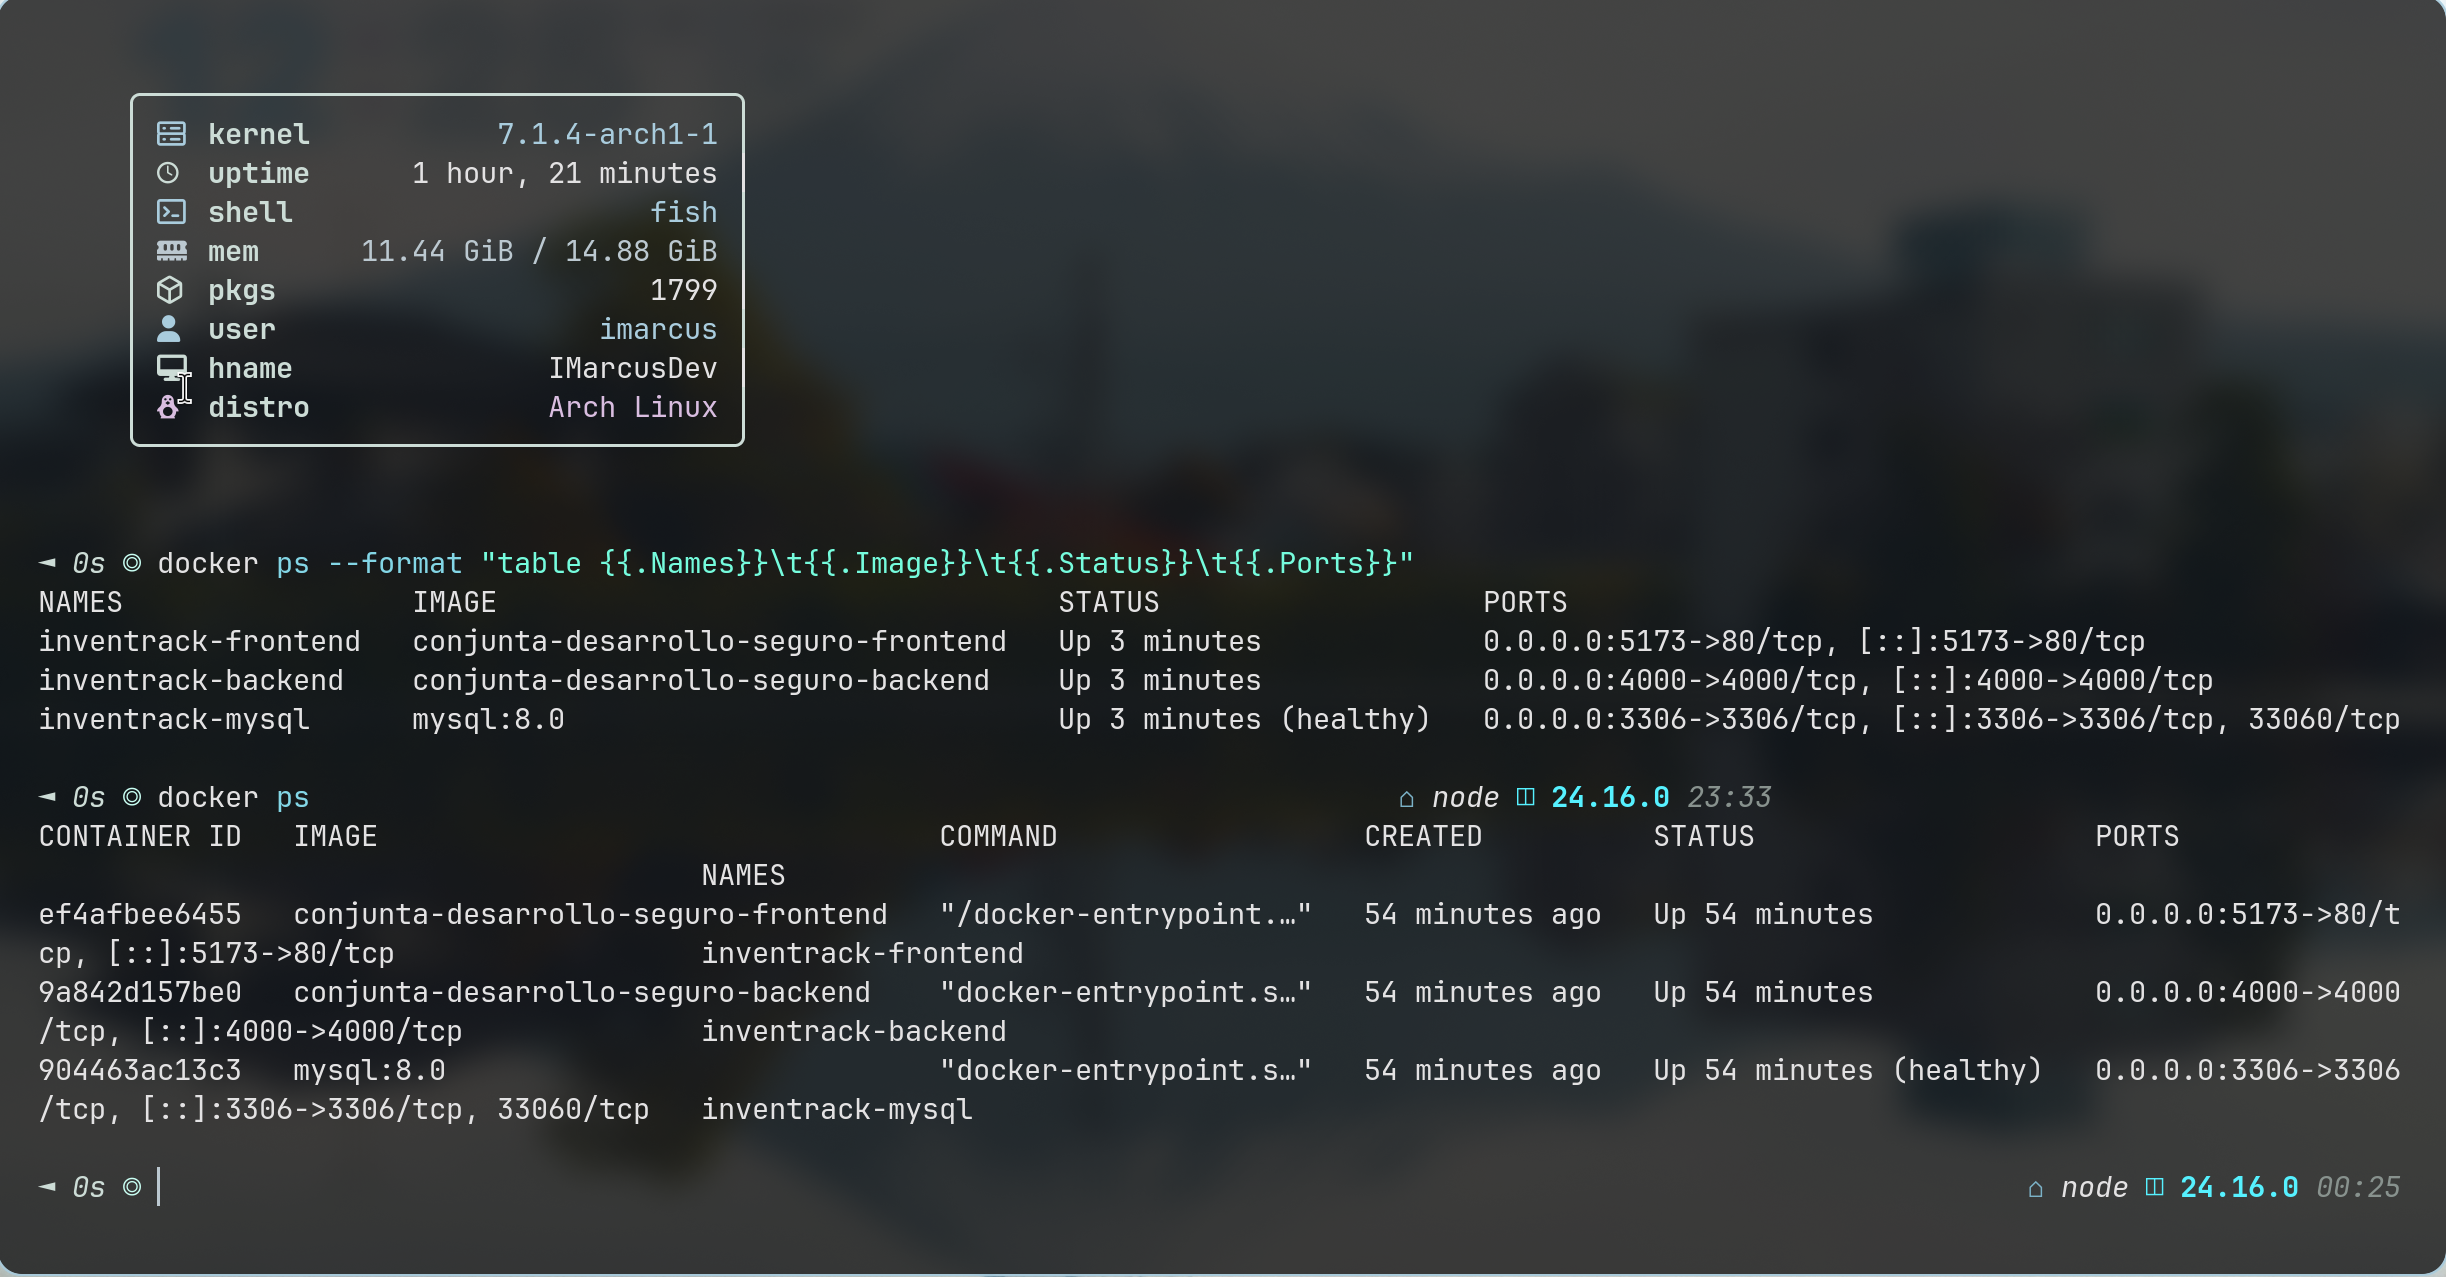
\includegraphics[width=1\linewidth]{contenedores_corriendo.png}
  \caption{Contenedores en ejecución (\texttt{docker ps}).}
  \label{fig:contenedores}
\end{figure}

%=====================================================================
% 2. MANIFIESTOS DE KUBERNETES (10%)
%=====================================================================
\section{Manifiestos de Kubernetes}

\subsection{Namespaces}

\subsection{Deployments y Services}

\subsection{ConfigMaps y Secrets}

\subsection{PersistentVolumeClaim (PVC)}

\subsection{Ingress}

%=====================================================================
% 3. DESPLIEGUE EN CLÚSTER Y CONFIGURACIÓN DE INGRESS (10%)
%=====================================================================
\section{Despliegue en el Clúster y Configuración de Ingress}

\subsection{Descripción del Clúster}
% Minikube / Kind / nube. >>> LLENAR <<<

\subsection{Controlador Ingress}
% Nginx Ingress Controller u otro. >>> LLENAR <<<

\subsection{Resolución del Dominio conjunta3p.espe.edu.ec}
% Justificar cómo se resolvió el DNS o el uso del archivo /etc/hosts.
\begin{lstlisting}[language=bash,caption={Configuración de /etc/hosts para el entorno de prueba},label=lst:hosts]
# >>> Ejemplo: 192.168.49.2   conjunta3p.espe.edu.ec <<<
\end{lstlisting}

\subsection{Evidencia: Recursos en Kubernetes}
\begin{figure}[H]
  \centering
  % 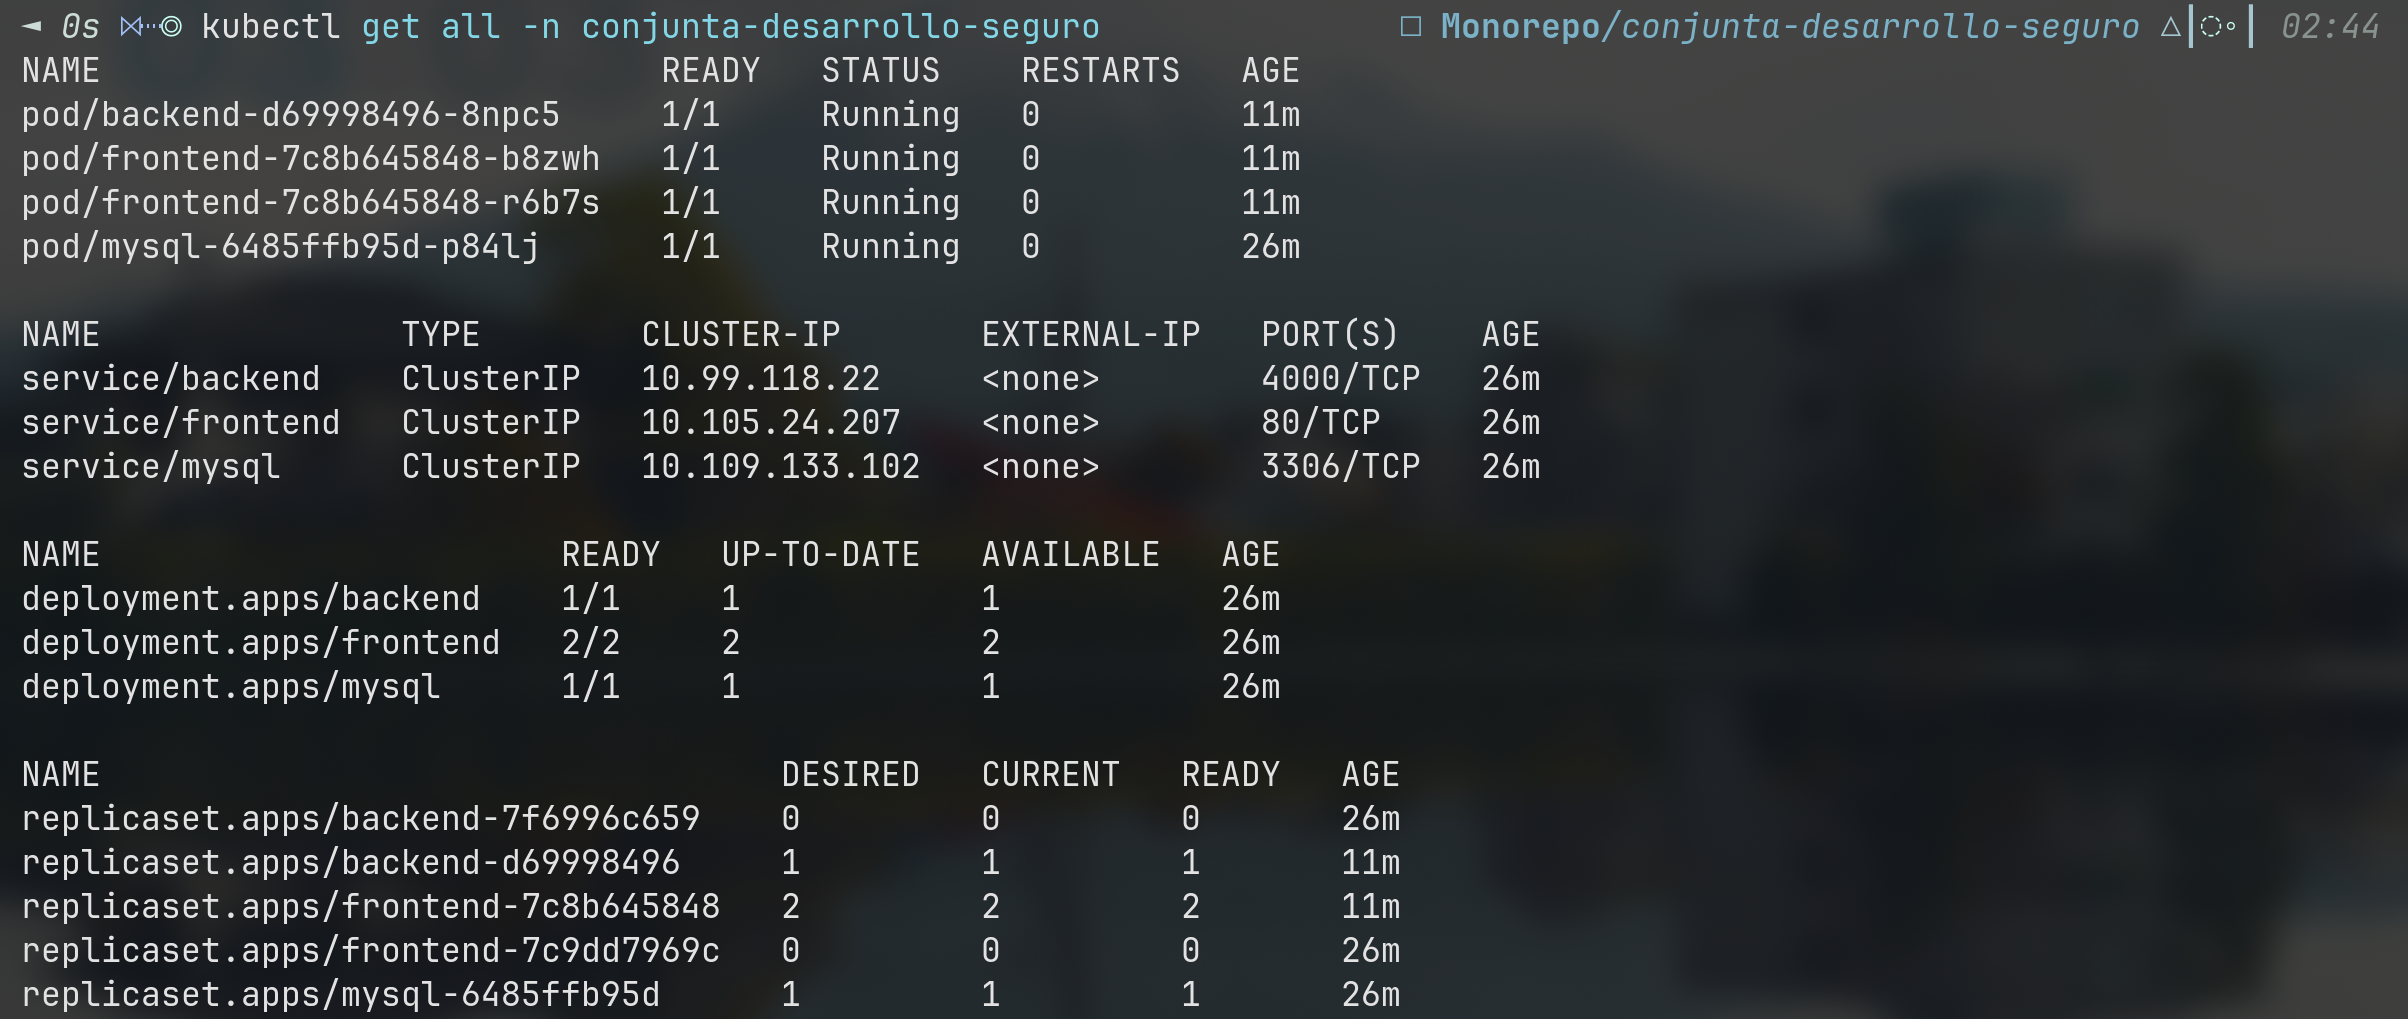
\includegraphics[width=0.9\textwidth]{kubectl_get_all.png}
  \caption{Pods, Services e Ingress en ejecución (\texttt{kubectl get all}).}
  \label{fig:kubectlall}
\end{figure}

\subsection{Evidencia: Aplicación en el Navegador}
\begin{figure}[H]
  \centering
  % 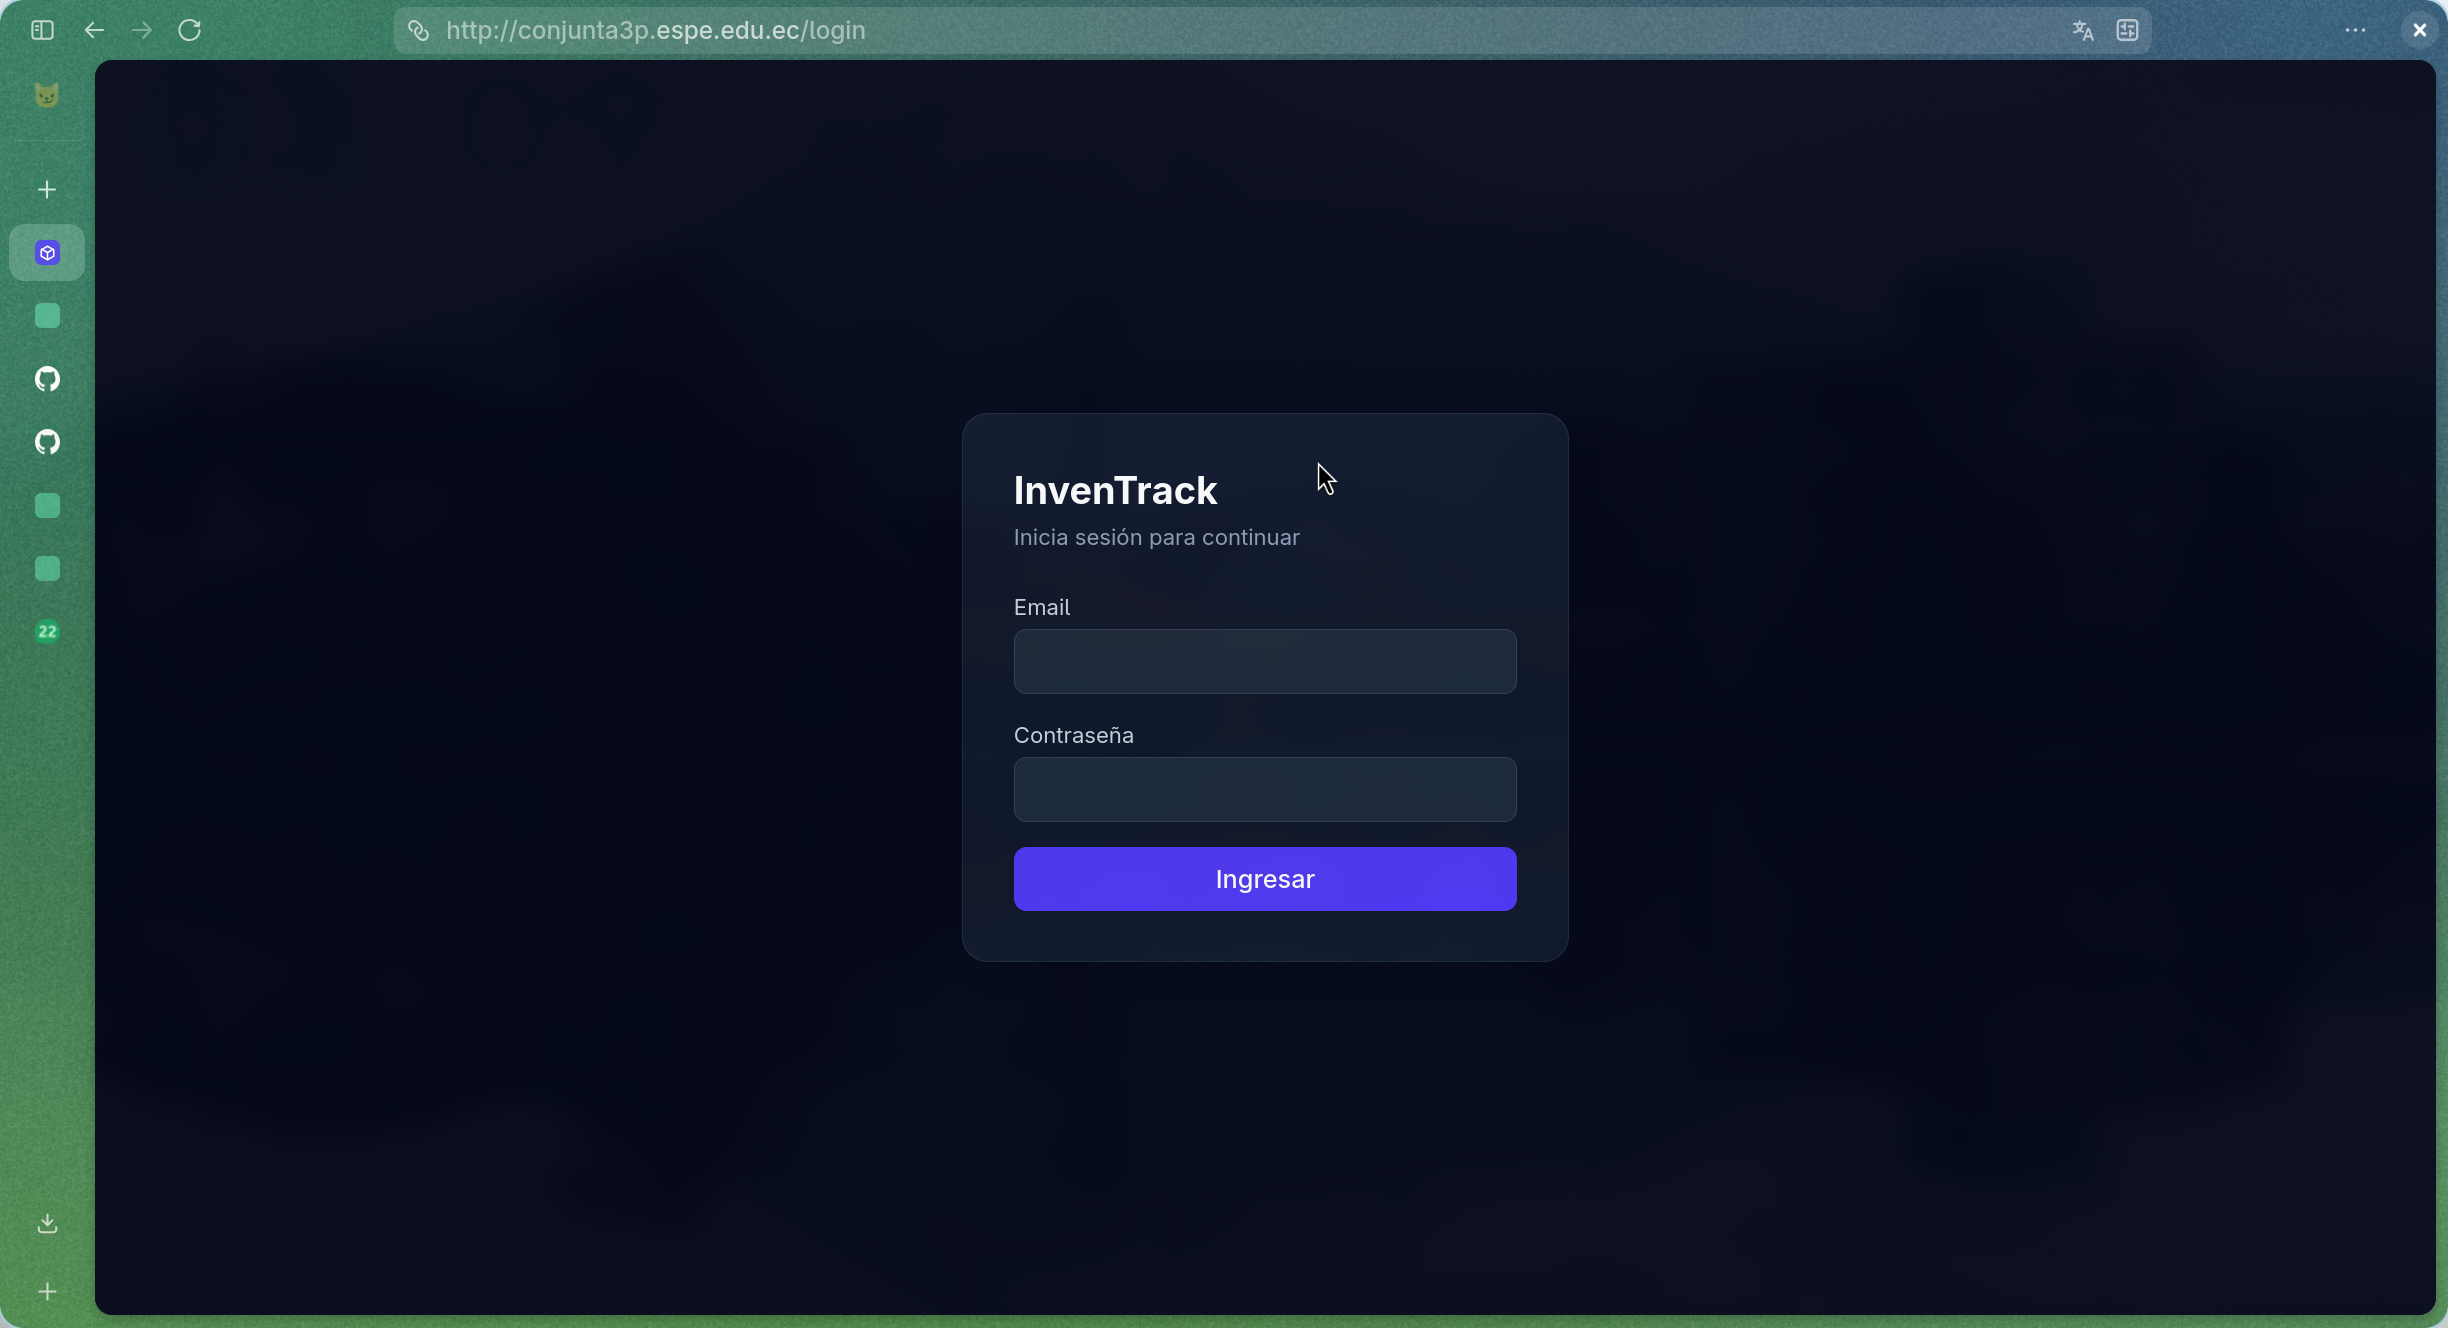
\includegraphics[width=0.9\textwidth]{navegador_dominio.png}
  \caption{InvenTrack accesible bajo el dominio \texttt{conjunta3p.espe.edu.ec}.}
  \label{fig:navegador}
\end{figure}

%=====================================================================
% 4. AUDITORÍA DE SEGURIDAD — PENTESTING PTES (60%)
%=====================================================================
\section{Auditoría de Seguridad: Pentesting con Metodología PTES}
% Introducción al proceso de pentesting sobre InvenTrack con Kali Linux.

%----------------------- FASE 1 -----------------------
\subsection{Fase 1: Interacciones Preliminares (Pre-engagement) — 5\%}
% Alcance, objetivos, restricciones, reglas de juego y autorizaciones.

\subsubsection{Alcance del Pentesting}
% >>> LLENAR <<<

\subsubsection{Objetivos y Reglas de Juego}
% >>> LLENAR <<<

\subsubsection{Activos a Probar}
% API backend, MySQL, JWT, chatbot IA. >>> LLENAR <<<

\subsubsection{Autorización}
% Declaración de autorización para la prueba. >>> LLENAR <<<

%----------------------- FASE 2 -----------------------
\subsection{Fase 2: Recopilación de Inteligencia (Intelligence Gathering) — 8\%}
% Información pasiva y activa: puertos, rutas de Ingress, cabeceras HTTP, tecnologías.

\subsubsection{Mapeo de Puertos (Nmap)}
\begin{lstlisting}[language=bash,caption={Comando Nmap ejecutado},label=lst:nmap]
# nmap -sV -p- conjunta3p.espe.edu.ec
# >>> PEGAR COMANDO Y RESULTADO <<<
\end{lstlisting}
\begin{figure}[H]
  \centering
  % \includegraphics[width=0.9\textwidth]{nmap.png}
  \caption{Resultado del escaneo de puertos con Nmap.}
  \label{fig:nmap}
\end{figure}

\subsubsection{Detección de Tecnologías (WhatWeb / Wappalyzer)}
% >>> LLENAR + captura <<<

\subsubsection{Cabeceras HTTP y Rutas de Ingress}
% >>> LLENAR + captura <<<

%----------------------- FASE 3 -----------------------
\subsection{Fase 3: Modelado de Amenazas (Threat Modeling) — 7\%}
% Activos críticos, vectores de ataque y superficies de exposición.

\begin{table}[H]
  \centering
  \caption{Matriz de modelado de amenazas de InvenTrack}
  \label{tab:threatmodel}
  \begin{tabularx}{\textwidth}{l X X}
    \toprule
    \textbf{Activo} & \textbf{Vector de Ataque} & \textbf{Superficie de Exposición} \\
    \midrule
    % >>> LLENAR las celdas de cada fila <<<
    API REST         & & \\
    Autenticación JWT & & \\
    Carga de archivos (Multer) & & \\
    Carga masiva Excel/CSV & & \\
    Chatbot (Groq)   & & \\
    Base de datos MySQL & & \\
    \bottomrule
  \end{tabularx}
\end{table}

%----------------------- FASE 4 -----------------------
\subsection{Fase 4: Análisis de Vulnerabilidades (Vulnerability Analysis) — 12\%}
% Escaneo automatizado y manual: Nikto, OWASP ZAP, Burp Suite, Nuclei.

\subsubsection{Escaneo con Nikto}
\begin{lstlisting}[language=bash,caption={Comando Nikto ejecutado},label=lst:nikto]
# nikto -h https://conjunta3p.espe.edu.ec
# >>> PEGAR COMANDO Y RESULTADO <<<
\end{lstlisting}

\subsubsection{Escaneo con OWASP ZAP / Burp Suite}
% >>> LLENAR + capturas <<<

\subsubsection{Análisis de Cabeceras de Seguridad}
% >>> LLENAR: HSTS, CSP, X-Frame-Options, etc. <<<

\subsubsection{Resumen de Vulnerabilidades Detectadas}
\begin{table}[H]
  \centering
  \caption{Vulnerabilidades detectadas en la fase de análisis}
  \label{tab:vulns}
  \begin{tabularx}{\textwidth}{l X l}
    \toprule
    \textbf{ID} & \textbf{Descripción} & \textbf{Severidad (CVSS)} \\
    \midrule
    % >>> LLENAR las celdas de cada fila <<<
    V-01 & & \\
    V-02 & & \\
    V-03 & & \\
    \bottomrule
  \end{tabularx}
\end{table}

%----------------------- FASE 5 -----------------------
\subsection{Fase 5: Explotación (Exploitation) — 15\%}
% Bypass de autenticación, fuerza bruta (rate limiting), inyección SQL, IDOR.

\subsubsection{Intento de Bypass de Autenticación}
% >>> LLENAR: procedimiento, payloads, resultado <<<

\subsubsection{Fuerza Bruta contra el Login (Hydra / Burp Intruder)}
\begin{lstlisting}[language=bash,caption={Comando de fuerza bruta ejecutado},label=lst:hydra]
# hydra -l admin -P rockyou.txt conjunta3p.espe.edu.ec http-post-form ...
\end{lstlisting}

\subsubsection{Inyección SQL (Login / Chatbot)}
% >>> LLENAR: payloads probados y resultado <<<

\subsubsection{Pruebas de IDOR (Endpoints de Auditoría / Kardex)}
% >>> LLENAR <<<

%----------------------- FASE 6 -----------------------
\subsection{Fase 6: Post-Explotación (Post-Exploitation) — 8\%}
% Impacto: acceso a datos sensibles, escalación de privilegios, extracción de datos,
% persistencia de sesión y validación del hasheo con bcrypt.

\subsubsection{Análisis de Impacto}
% >>> LLENAR <<<

\subsubsection{Validación del Hasheo con bcrypt}
% >>> LLENAR <<<

\subsubsection{Escalación de Privilegios (admin vs almacenero)}
% >>> LLENAR <<<

%----------------------- FASE 7 -----------------------
\subsection{Fase 7: Reporte (Reporting) — 5\%}
% Hallazgos clasificados por severidad (CVSS), evidencias y recomendaciones.

\subsubsection{Clasificación de Hallazgos por Severidad}
\begin{table}[H]
  \centering
  \caption{Hallazgos clasificados por severidad CVSS}
  \label{tab:hallazgos}
  \begin{tabularx}{\textwidth}{l X l l}
    \toprule
    \textbf{ID} & \textbf{Hallazgo} & \textbf{CVSS} & \textbf{Severidad} \\
    \midrule
    % >>> LLENAR las celdas de cada fila <<<
    H-01 & & & \\
    H-02 & & & \\
    H-03 & & & \\
    \bottomrule
  \end{tabularx}
\end{table}

\subsubsection{Validación de Controles de Seguridad}
% Rate limiting, bcrypt, JWT, verificación de sesión cada 5s.
% Documentar cuáles resultaron efectivos y cuáles fallidos.
\begin{table}[H]
  \centering
  \caption{Validación de controles de seguridad de InvenTrack}
  \label{tab:controles}
  \begin{tabularx}{\textwidth}{l X l}
    \toprule
    \textbf{Control} & \textbf{Prueba Realizada} & \textbf{Resultado} \\
    \midrule
    % >>> LLENAR las celdas de cada fila <<<
    Rate limiting & & \\
    Hasheo bcrypt & & \\
    Tokens JWT & & \\
    Verificación de sesión (5s) & & \\
    \bottomrule
  \end{tabularx}
\end{table}

%=====================================================================
% 5. CONCLUSIONES Y RECOMENDACIONES
%=====================================================================
\section{Conclusiones y Recomendaciones}

\subsection{Conclusiones}
% >>> LLENAR <<<

\subsection{Recomendaciones de Mejora para InvenTrack}
\begin{itemize}
  \item % >>> LLENAR: recomendaciones accionables <<<
  \item
  \item
\end{itemize}

%=====================================================================
% REFERENCIAS (APA 7)
%=====================================================================
\printbibliography[title={Referencias}]

%=====================================================================
% APÉNDICES
%=====================================================================
\appendix
\section{Apéndice A: Evidencias Adicionales}
% Capturas de pantalla, logs extensos o payloads completos.
% >>> LLENAR (opcional) <<<

\end{document}
